% \cleardoublepage

% \section{Overleaf 使用注意事项}

% 如果你在Overleaf上编译本模板,请注意如下事项~\cite{zjuthesis}:

% \begin{itemize}
%     \item 删除根目录的 ``.latexmkrc'' 文件,否则编译失败且不报任何错误
%     \item 字体有版权所以本模板不能附带字体,请务必手动上传字体文件,并在各个专业模板下手动指定字体。
%         具体方法参照 GitHub 主页的说明。
%     \item 当前(2019年9月2日)的Overleaf使用TexLive 2017进行编译,但一些伪粗体复制乱码的问题需要TexLive 2019版本来解决。
%         所以各位同学可以在Overleaf上编写论文,但务必使用本地的TexLive 2019来进行最终编译,以免产生查重相关问题。
%         具体说明参照 GitHub 主页。
% \end{itemize}

% \subsection{节标题}

% \subsubsection{小节标题}   %2.1

% \par 我们可以用includegraphics来插入现有的jpg等格式的图片,如\autoref{fig:zju-logo}。

% \begin{figure}[ht]
%     \centering
%     
\includegraphics[width=.4\linewidth]{logo/zju}
%     \caption{\label{fig:zju-logo}浙江大学LOGO}
% \end{figure}

% \par 如\autoref{tab:sample}所示,这是一张自动调节列宽的表格。

% \begin{table}[ht]
%     \caption{\label{tab:sample}自动调节列宽的表格}
%     \begin{tabularx}{\linewidth}{|c|X<{\centering}|}
%         \hline
%         第一列 & 第二列 \\ \hline
%         xxx & xxx \\ \hline
%         xxx & xxx \\ \hline
%         xxx & xxx \\ \hline
%     \end{tabularx}
% \end{table}

% \par 如\autoref{equ:sample},这是一个公式

% \begin{equation}
%     \label{equ:sample}
%     A=\overbrace{(a+b+c)+\underbrace{i(d+e+f)}_{\text{虚数}}}^{\text{复数}}
% \end{equation}

% \par 如\autoref{code:sample}所示,这是一段代码。
% 计算机学院的代码样式可能与其他专业不同,
% 如有需要,可以从计算机学院专业模板中复制相关的代码样式设定。

% \begin{lstlisting}[%
%     language={C},
%     caption={simple.c},
%     label={code:sample}
% ]
% #include <stdio.h>

% int main(int argc, char *argv[])
% {
%     printf("Hello, zjuthesis\n");
%     return 0;
% }
% \end{lstlisting}





% \subsection{关于字体}      %2.2

% 英文字体通常提供了粗体和斜体的组合,中文字体通常没有粗体或斜体,本模板使用了 `AutoFakeBold' 来实现中文伪粗体,但不提供中文斜体,如\autoref{tab:font-examples}所示。

% \begin{table}
%     \centering
%     \caption{一些字体示例}
%     \label{tab:font-examples}
%     \begin{tabular}{|c|c|c|c|c|}
%         \hline
%         字体            & 常规             & 粗体                       & 斜体                      & 粗斜体                                \\ \hline
%         Times New Roman & Regular         & {\bfseries          Bold} & {\itshape         Italic} & {\bfseries \itshape      BoldItalic} \\ \hline
%         仿宋            & {\fangsong 常规} & {\fangsong \bfseries 粗体} & {\fangsong \itshape 斜体} & {\fangsong \bfseries \itshape 粗斜体} \\ \hline
%         宋体            & {\songti   常规} & {\songti   \bfseries 粗体} & {\songti   \itshape 斜体} & {\songti   \bfseries \itshape 粗斜体} \\ \hline
%         黑体            & {\heiti    常规} & {\heiti    \bfseries 粗体} & {\heiti    \itshape 斜体} & {\heiti    \bfseries \itshape 粗斜体} \\ \hline
%         楷体            & {\kaishu   常规} & {\kaishu   \bfseries 粗体} & {\kaishu   \itshape 斜体} & {\kaishu   \bfseries \itshape 粗斜体} \\ \hline
%     \end{tabular}
% \end{table}

% \sectionnonum[none]{同一页上的章标题}


%%%%%%%%%%%%%%%%%%%%%%%%%%%%%%%%%%%%%%%%%%%%%
%%%%%%%%第2章 自动化根因分析相关技术研究%%%%%%%
%%%%%%%%%%%%%%%%%%%%%%%%%%%%%%%%%%%%%%%%%%%%%

\section{自动化根因分析相关技术研究}        %第2章
\subsection{概述}
在科学和工程学中,根因分析是一种解决问题的方法,用于识别故障或问题的根本原因。
它广泛应用于IT运营、电信、工业过程控制、事故分析、医学等。
根因分析通常是一种系统性的过程,需要收集和分析与问题相关的数据和信息,运用各种工具和技术来确定问题的根本原因。
在计算机领域,特别是在软件安全领域,根因分析通常是指分析软件或系统崩溃的根本原因,它可能涉及对系统的代码、设计、配置、环境等方面进行深入分析。
通过根因分析,开发团队可以更好地了解程序中的潜在问题,并及时采取措施修复和加固系统,以提高软件的安全性和稳定性。
作为一种粗略的可靠性度量方法,模糊测试可以针对待分析程序产生不同输入得到程序崩溃,并提示程序哪些部件需要特殊的注意;
而根因分析作为模糊模糊测试的后续阶段,可以利用,模糊测试得到的已知崩溃进行深入分析并找出导致这些问题的根本原因。
%此处要插入一个自动化根因分析方法的概述图
一般来说,当前自动化根因分析方法主要包括两类:基于频谱的根因分析方法和基于事后的根因分析方法。
其中基于频谱的方法通常在初始崩溃测试用例的基础上生成两大组崩溃测试用例和非崩溃测试用例。
它们记录每条指令上的寄存器和内存数据,以统计方式构建崩溃的必要条件作为谓词,测量每个谓词与初始崩溃的相关性,最后将谓词列为根本原因;
而基于事后的故障定位方法从调试文件(例如核心转储和内存快照)开始,执行反向执行和向后污染分析,以跟踪无效数据的传播。
它们分析指令的语义,比基于频谱的故障定位方法更有效。
同时,随着当前AI领域的发展,机器学习的长足发展与大模型的出现使根因分析进入了新的维度,一些繁杂的人工工作可以交由AI辅助进行。
这极大提高了一些受到时间和复杂程度限制方法的效率,拓宽了根因分析领域

下面将从这三个方面介绍自动化根因分析相关技术的研究
\subsection{自动化根因分析相关方法}
%下面三个要分别插入一个类别的论文的方法图
\subsubsection{基于频谱的自动化根因分析方法}
基于频谱的分析方法是一种利用软件系统的执行频谱(Execution Spectrum)来识别和定位问题的技术。
该方法通常用于识别性能问题和资源利用不足等情况。
基本原理是在软件运行时记录系统的执行轨迹或事件,然后通过分析这些事件的频率和模式来识别可能的瓶颈或问题。
基于频谱的故障定位技术基于一个核心假设:程序中出错频率较高的部分更有可能是故障所在。
这种方法使用“频谱”信息,即程序执行过程中各个组件(如函数、语句或分支)的执行频率和失败频率的统计数据。
例如,对于性能问题,可以记录系统中的函数调用、代码路径执行次数、资源利用情况等信息。
通过分析这些数据,可以确定哪些函数或路径是性能瓶颈,并识别可能的优化方向。
这种方法可以帮助开发人员了解系统的执行特征,并优化系统的性能和资源利用率。
大多数基于频谱的根因分析技术研究侧重于统计量的设计,包括排名指标和分布统计。
但也有一些工作侧重对测试用例的研究:
Hao等人~\cite{Test2010}根据测试用例的能力提出了三种减少测试用例数量的策略,基于使用测试输入的测试运行的执行跟踪,使开发人员可以只选择测试输入的一个有代表性的子集来进行结果检查和故障定位;
Abreu等人~\cite{practical2009}通过使用由西门子集和空间程序组成的通用基准,研究了作为多个参数(例如系统执行期间收集的程序频谱的质量和数量)的函数的诊断准确性,结果表明用于分析程序谱的特定相似系数的优越性能在很大程度上独立于测试设计,并且证明了SFL可以有效地应用于工业环境中的嵌入式软件开发环境中;
Dandan Xu等人~\cite{Racing}设计并实现了一种反例强化学习技术,该技术奖励涉及反例的操作,通过平衡随机抽样和对反例的利用,利用每个模糊测试回合的结果来指导下一轮模糊测试,从而将当今基于频谱的根因分析工具的可扩展性和准确性提高了一个数量级以上。

\subsubsection{基于事后的故障定位方法}
基于事后的根因分析技术是一种在崩溃发生后开始的根因分析技术。
该方法的基本原理是通过收集和分析系统状态、日志、内存转储等信息,来确定问题的根本原因和触发条件。
通过分析这些信息,可以确定程序的内存泄漏、空指针引用等异常行为,并采取措施修复或预防类似问题的再次发生。
在事后程序分析技术中,记录与重放~\cite{ReCrash2008}~\cite{SymCrash2014}~\cite{Chronicler2013}和核心转储分析~\cite{RETracer2016}~\cite{Making2015}~\cite{CREDAL2016}是两种常见方法。

\textbf{记录与重放}\ 这种方法的核心思想是在程序运行时使用工具捕获程序的执行轨迹和状态,从而允许开发者在出现故障时能够准确重现问题。
在程序执行过程中,记录所有导致状态变化的事件,包括函数调用、外部输入、线程操作和其他系统调用等事件。
之后利用捕获的这些事件的参数和结果,以及它们的时间戳和执行顺序进行事后分析,找到导致崩溃的根因。
值得注意的是通常“记录”过程需要通过修改操作系统的内核、使用特定的库或工具、或者插桩代码来实现;同时“重放”过程通常需要在一个控制的环境中进行,以避免非确定性行为的干扰。
这种方法存在着局限性:(1)记录阶段可能会引入显著的时间和空间开销,特别是在需要详尽记录的情况下。
(2)无法重放某些不确定性较高的行为:如并发和竞争条件漏洞导致的崩溃就可能在重放时难以精确复现。

\textbf{核心转储分析}\ 与记录与重放方法不同,核心转储分析方法涉及捕捉程序崩溃时的内存镜像,以便分析和诊断导致崩溃的原因。
这种技术对于理解复杂软件系统的失败原因非常有用,特别是在调试难以复现的故障时体现出了较大的优势。
核心转储方法的基本原理是当程序异常终止(如段错误)发生崩溃时,自动保存那部分程序执行时的内存内容。
这个转储文件包含了程序终止时的变量值、程序计数器、寄存器内容、堆栈信息等关键数据。
发生崩溃后,分析者通过检查崩溃时的内存状态,分析崩溃的上下文,确定崩溃发生在程序的哪一部分。
这种方法存在着一定的局限性:(1)核心转储文件可能非常大,尤其是密集应用内存的程序,这可能极大提高分析的开销。
(2)某些崩溃依赖于程序运行的特定环境或状态,单纯利用核心转储文件无法分析导致崩溃的原因。


虽然当前这些研究被证明是有效的,但它们只关注特定的类型状态问题,或者在反向执行时难以解决内存别名等问题,仍然不足够高效。
\subsubsection{基于机器学习的自动化根因分析方法}
这种方法利用机器学习算法来自动识别和诊断系统故障的根本原因,并依赖于历史数据和模式识别技术来预测和识别问题的根源。这种方法在处理复杂系统和大规模数据时显示出其独特的优势。
通过分析系统的正常运行数据和故障时的数据,机器学习模型可以学习到哪些指标或事件与系统故障强相关。
在基于机器学习的自动化根因分析方法中,首先收集系统的运行日志、性能指标、系统事件等数据;
其次从原始数据中提取有用的特征如CPU使用率、内存使用量、响应时间、错误率等,这些特征能够代表系统的运行状态或可能影响系统性能和稳定性的因素;
之后利用其训练机器学习模型,并在实际数据上运行模型,以检测和预测潜在的系统故障。
这种方法也存在着一定的局限性:(1)模型的效果很大程度上依赖于高质量和高覆盖率的数据,需要人工提供较为优质的训练数据。(2)模型需要不断维护、微调与更新,从而能在快速变化的系统环境中适应新的数据和条件。
图n展示了ModelCoder~\cite{9521318}这一基于机器学习的自动化根因分析方法的实现过程:

\subsection{其他相关研究}
\subsubsection{逆向执行}
在基于事后分析的故障定位领域,分析人员通过反向执行来更深入地了解程序崩溃~\cite{RETracer2016}~\cite{REPT}。
反向执行是一种通过撤销已执行的指令,恢复寄存器和内存值到先前状态的技术,使分析人员能够从独特的视角观察程序状态随时间的演变过程。
这需要分析人员设计复杂的处理器,根据指令的行为逆向执行指令。
在本文关注的嵌入式固件领域,目标硬件平台的资源受限性质通常严重限制了监控和记录能力,导致无法获取足够的数据以支持全面的反向执行。
为了解决这一问题,需要设计合理的运行时记录方法,并为嵌入式固件设计合适的逆向处理器。

\subsubsection{使用——定义链}
在数据流分析领域,使用——定义链(Use-Define Chain)是一种描述程序中一个变量的使用和所有定义的数据结构,该变量可以在没有任何其他中间定义的情况下到达使用~\cite{Compilers2007}。
使用定义链建立了程序中变量的定义点(定义变量值的地方)与使用点(使用这些变量值的地方)之间的关系。
通过这种结构,分析人员可以追踪变量值是如何在程序中传递和转换的,从而可以提高逆向执行中的效率

\subsection{本章小结}
本章中,首先对根因分析方法进行了简单背景介绍,然后讨论了当前主流的几种自动化根因分析方法,并分析了他们的优势与不足。
最后补充分析了自动化根因分析方法中逆向执行和使用——定义链等其他相关研究。

%%%%%%%%%%%%%%%%%%%%%%%%%%%%%%%%%%%%%%%%%%%%%
%%%%%%%%第3章 物联网嵌入式固件自动化根因分析%%%
%%%%%%%%%%%%%%%%%%%%%%%%%%%%%%%%%%%%%%%%%%%%%

\section{物联网嵌入式固件自动化根因分析}    %第3章
\subsection{引言}                         %3.1节
随着网络技术的飞速发展,物联网技术的应用已经渗透到各个产业领域。
嵌入式固件在这些领域中起着关键作用,它使得设备和系统能够实现自动化、智能化的控制和管理,提高生产效率、节约资源、降低成本。
然而随着嵌入式固件深入生活各个领域,其中的漏洞与安全问题重要性愈发重要。
2023年12月,丰田雷克萨斯~\cite{toyota}由于发动机电子控制单元存在安全隐患,召回了超过十万辆车。
嵌入式固件安全在国防方面同样重要,俄乌战争中,Viasat的KA-SAT网络收到了攻击~\cite{KASAT},
攻击者利用卫星调制解调器固件的漏洞进行攻击,导致KA-SAT的卫星宽带服务部分中断,影响了数千名客户和5800台风力涡轮机的远程访问。

目前模糊测试领域已有较为成熟的方法来检测固件漏洞,但在模糊测试发生崩溃后,需要进一步进行根因分析导致崩溃的原因,修复漏洞。
目前已有几种主流的自动化根因分析方法。
但目前尚未有针对嵌入式固件的自动化根因分析方法。由于嵌入式固件运行时资源受限,以及代码缺乏必要的调试信息,导致在固件领域已有的自动化分根因析方法难以有效分析导致崩溃的根本原因;
而手动分析较为繁琐,且由于人工难以理解二进制固件代码,难以全面分析,并高覆盖率发现bug。

综上所述,如何针对物联网嵌入式固件实现高效自动化根因分析方法,发现固件漏洞,保障物联网嵌入固件安全,是当前亟需解决的问题。

\subsection{本文研究的问题定义}             %3.2节
\subsubsection{本文关注的根本原因}          %3.2.1节
现实世界中的固件崩溃原因多种多样且复杂,如使用后释放(use after free)、双重释放(double free)和越界写入(out-of-bounds write)。
然而,大多数固件崩溃的原因是两个:无效的内存访问和无效的指令执行。
因为它们直接关系到程序的基本执行和内存管理机制,尤为重要,是所有计算系统都必须妥善处理的基本安全和稳定性挑战,解决这类漏洞是提高固件质量和系统安全的关键。
本文选取这两个漏洞进行重点分析,将导致固件崩溃的根因定义为这两种漏洞。

\textbf{无效的内存访问}\ 无效的内存访问是指程序试图访问其没有权限访问的内存区域,主要包括以下几种:
(1)越界访问:程序试图访问数组、字符串或其他数据结构的边界之外的内存;
(2)野指针访问:未初始化或已释放的指针被错误地用于内存访问;
(3)空指针解引用:程序试图通过一个指向NULL的指针访问内存或访问已经被释放的内存块。
这些无效内存访问会触发操作系统的保护机制,如分页错误(page fault)或访问违规(access violation),从而导致程序崩溃或终止。
同时也可能导致数据损坏或被恶意代码利用。

\textbf{无效的指令执行}\ 无效的指令执行通常指的是程序试图执行非法或非预期的机器指令。通常由以下情况几种引起:
(1)代码损坏:程序代码由于某种原因(如内存损坏、磁盘故障、恶意攻击等)被更改,导致执行流程跳转到非法的指令上;
(2)函数指针错误:错误的函数指针可能导致程序跳转到错误的地址执行,尤其是在使用动态链接库(DLL)或回调函数时;
(3)类型错误:程序错误解析了变量类型,或应用了不匹配的类型,如将整数用作函数指针,可能导致程序尝试执行数据区域的代码。
执行无效指令可能导致程序行为不可预测,从错误操作到程序崩溃都可能发生,严重时可能被用于执行恶意代码,是一种较为常见但是又较为危险的漏洞

\subsubsection{内存别名问题}                %3.2.2节
在分析固件崩溃的原因时,分析人员需要通过逆向分析执行轨迹,通过逆向导致崩溃过程的指令,来分析出导致崩溃的根本原因。
这一过程涉及对崩溃前的数万条指令的深入分析,以追踪数据的流向和变化。
在分析导致固件崩溃的执行轨迹时,需要重点考虑故障定位中的一个常见而关键的问题——内存别名问题。
该问题描述的是多个指针可能指向同一块底层内存位置,在逆向时无法确定是哪个指针导致了内存的改变。
这种情况增加了数据流分析的不确定性,并且复杂化了准确追踪数据传播的任务~\cite{REPT}~\cite{RETracer2016}。

\begin{lstlisting}[%
    language={asm},
    caption={内存别名问题示例},
    label={code_alias}
]
; 假设edi寄存器存储的是某个对象的地址
mov eax, [edi + 4]  ; 从对象中加载第一个字段到 eax
add eax, 10         ; 对该字段增加10
mov [edi + 4], eax  ; 将修改后的值写回相同位置

; esi寄存器通过计算得到相同的内存地址
lea esi, [edi + 4]  ; 加载相同的内存地址到 esi
mov ebx, [esi]      ; 加载数据到 ebx,期望得到原始数据
\end{lstlisting}

具体地,\autoref{code_alias}是一个内存别名的简单例子,在这个例子中,$edi+4$和$esi$实际上指向同一内存位置,$eax$通过$edi + 4$加载和存储数据,而$ebx$通过$esi$来加载数据。
虽然$edi+4$和$esi$指向同一地址,但途径不同,这会使逆向工程师或者自动化工具误为这两个操作影响的是两个独立的内存区域;
也会导致我们无法分析出内存的改变是哪个指针做出的,这对代码分析影响极为严重,甚至可能导致巨大的性能下降。
此外,在并发编程中,内存别名会增加数据竞态的风险。

因此,内存别名作为一项重要的问题,需要在自动化方法设计中特备关注。

\subsection{物联网嵌入式固件自动化根因分析方法设计} %3.3节
针对嵌入式固件运行时资源有限以及调试信息有限的特点,我们提出了如~\autoref{fig:overview}所示的自动化根因分析框架。
\begin{figure}[h]
    \centering
    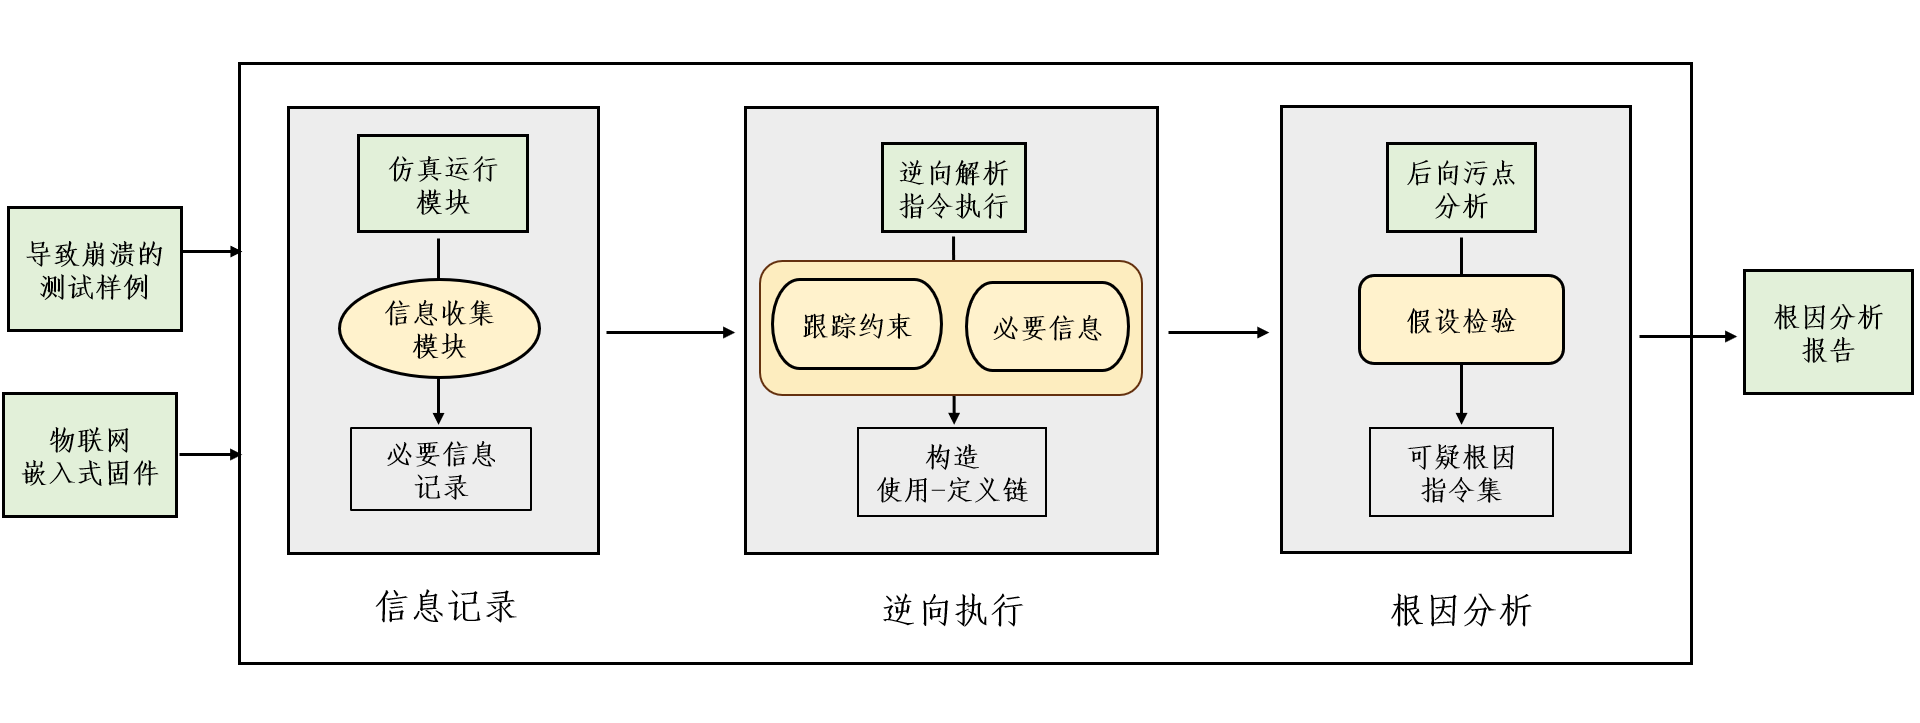
\includegraphics[width=1.0\textwidth]{./figure/Overview.png}
    \caption{物联网嵌入式固件自动化根因分析方法框架}
    \label{fig:overview}
\end{figure}\\
本方法通过三个主要组件实现高效精准的崩溃分析:
首先是高效运行时信息记录组件,在此阶段,系统通过模拟执行引起崩溃的测试用例来收集关键的运行时数据;
之后是历史信息指导的逆向执行组件,此阶段利用记录的数据解决内存别名问题,确保数据流分析的准确性;
最后进行根因分析组件,通过后向污点分析确定导致崩溃的具体原因,为进一步的调查提供指导。
这一整体架构能够在资源受限的环境中有效地定位固件中的错误和安全漏洞。

\subsubsection{高效运行时信息记录}
为了有效地分析固件崩溃,解决在资源受限的固件环境中调试机制不足的问题,本设计引入了一种高效的运行时信息记录的方法。
本方法首先执行带有崩溃测试用例的固件二进制文件,并收集运行时数据,如寄存器状态和内存访问等,以支持随后的反向执行和根本原因分析。

为了分析固件崩溃,本方法主要识别了一种关键的事件类型:内存读取与写入。
这些事件涉及到内存的读取和写入操作,如内存访问,寄存器操作等。
内存读写事件在后续追踪中,可以有效辅助分析崩溃过程中数据是如何被处理和转移的。
系统利用固件重置技术来执行崩溃测试用例,同时监控和记录内存读写。
\begin{lstlisting}[
    language={asm},
    caption={内存读取与写入事件示例},
    label={code_memacc}
]
0x403b76 STR R0, [R3, #16]      ;(a)R0:0x0, R3:0x201073c4
0x403b78 LDR R9, [R5, #16]
…
0x406c78 LDR R6, [R0, #16]      ;(b)R0:0x201073c4, R6:0x0
0x406c7a LDR R4, [R6, #8]       ;(c)Crash!
\end{lstlisting}

如~\autoref{code_memacc}所示, 程序首先在地址$R3 + 16$处存储$R0$的值(指令a);
然后程序加载$R0 + 16$地址处的值并将其赋给$R6$(指令b),由于此处$R0$值与指令$a$处$R3$值相同,所以$R6$的值会变为$0x0$;
接着,程序试图从$R6 + 8$的地址加载值,由于$R6$此时为$0x0$,导致了空指针解引用的崩溃(指令c)。

这个例子展示了一个无效读取导致的崩溃。然而,在给定崩溃测试用例和固件二进制文件的情况下,获取此类崩溃知识并不是一件简单的事情。
分析人员需要深入研究运行时细节,检查从崩溃现场开始的每一条指令,最终确定$R0 + 16$和$R3 + 16$指向相同地址(即$0x201073d4$),
并且$R0$在(指令a)处的无效值(即$0x0$)引发了崩溃。

为了解决这种问题对根因分析造成的困扰,我们设计了一种高效的运行时信息记录方法。
首先我们在仿真环境模拟运行程序,在运行时主要关注两种类型的内存事件:(1)成功的内存读取和(2)成功的内存写入。
当任何一种事件发生时,本方法会暂停仿真,捕捉相关的运行时信息,如指令地址、操作的数据、寄存器状态以及内存地址等。
为了有效地保存和追踪这些事件,我们设计了一种特定的数据结构,用以记录内存访问的类型(读或写)、执行的指令地址、具体的数据内容、相应的内存地址以及寄存器的值。
%此处添加这个数据结构
借助这些数据事件,我们能够获得具体的内存访问信息,而非仅仅恢复寄存器和内存数据。
通过这种基于事件的方法,我们能够有效地构建出一幅详细的崩溃现场“画像”。
这样的信息收集为后续的逆向执行和根因分析提供了数据基础。
这种方法不仅提高了信息收集的效率,而且由于是在控制环境中进行,还增加了分析的可靠性和精确性。
\subsubsection{历史信息指导的逆向执行}
逆向执行阶段的主要目的是构建崩溃测试用例中数据的动态传播路径。
为了解决前文提到的可能会混淆数据流分析的普遍问题——内存别名,本方法采用了一种历史驱动的逆向执行方法。
这种方法通过利用在信息记录阶段捕获的具体内存访问信息,能够有效并准确地解决内存别名问题,从而使得数据依赖关系的追踪更加精确。
这种逆向执行策略增强了对数据传播路径的理解,提高了根因分析的精度和效率。

对于导致崩溃的无效内存访问或无效指令执行,确定根本原因的基本思路是从崩溃处开始逆向执行轨迹中的指令,以查明导致崩溃的数据为何被污染,这个过程被称为逆向执行。
然而,即便拥有完整的执行轨迹,精确地确定数据传播和相关联个别指令也是面临着较大的困难。
这主要是因为内存别名问题。例如,再考虑~\autoref{code_memacc}的例子,其中指令(a)和指令(b)访问相同的内存地址(即$0x201073d4$)。
如果我们能够建立这种关联,那么我们就可以将指令(a)视为崩溃的根本原因。
然而,主要困难在于这些指令涉及的具体内存地址常常由于不可逆指令的存在而变得模糊不清。
以指令$MOV\ R3,\ \#0$为例,它将寄存器$R3$设置为$0x0$,在逆向执行时我们只知道R3在这条指令被执行后的值是$0X0$,但无法恢复这条指令执行前$R3$的原始值。

\begin{figure}[h]
    \centering
    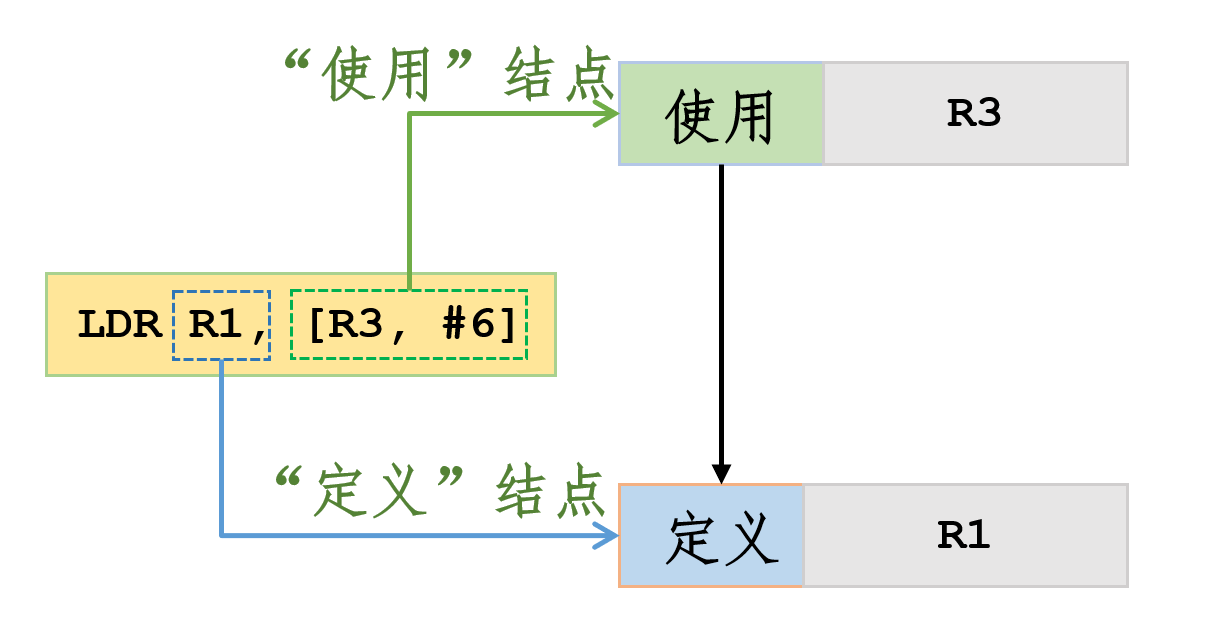
\includegraphics[width=1.0\textwidth]{./figure/UD-Chain.png}
    \caption{一个简单的使用定义链示例}
    \label{fig:ud-chain}
\end{figure}

为了应对这一难点,我们设计了一个历史信息指导的逆向执行方法。首先,我们构建使用-定义链来分析执行轨迹,此结构能帮助我们追踪每个操作的影响,明确数据是如何从一个操作传递到另一个操作的。
然后,在使用-定义链的基础上,我们进行了逆向执行指令以恢复寄存器到之前的状态。如~\autoref{fig:ud-chain}是一个简单的使用定义链示例。

\textbf{(1)使用——定义链构建}\ 这个过程从迭代重构完整执行轨迹开始,
对于遇到的每条指令,我们会仔细解析指令的行为,提取源操作数和目标操作数,这些操作数代表了指令内的数据流。
下面以~\autoref{code:udchain}所示的程序为例展示如何构建使用——定义链:
\begin{lstlisting}[
    language={asm},
    caption={构建使用——定义链过程代码示例},
    label={code:udchain}
]
MOV R1, #4      ; (a) 将数字4加载到寄存器R1
MOV R2, #10     ; (b) 将数字10加载到寄存器R2
ADD R3, R1, R2  ; (c) 将R1和R2的值相加,结果存入R3
STR R3, [R4]    ; (d) 将R3的内容存储到R4指向的内存地址
\end{lstlisting}

首先对于指令(a):$MOV\ R1,\ \#4$,涉及到的定义节点为$R1$。
对于指令(b):$MOV\ R2,\ \#10$,涉及到了对$R2$的定义。
对于指令(c):$ADD\ R3,\ R1, R2$,其中$R1$,$R2$的值被读取并用于计算,因此它们是使用节点;同时这条指令定义了$R3$的值,所以$R3$是一个定义节点。
对于指令(d):$STR\ R3,\ [R4]$,$R3$的值被用于存储操作,而$R4$是作为地址的基础,因此它们都是使用节点;
同时由于这个操作定义了内存地址$[R4]$的内容,所以$R4$是一个定义节点。
直观的,我们可以用\autoref{fig:viaual_udchain2}如所示来表述数据的流动。
\begin{figure}[h]
    \centering
    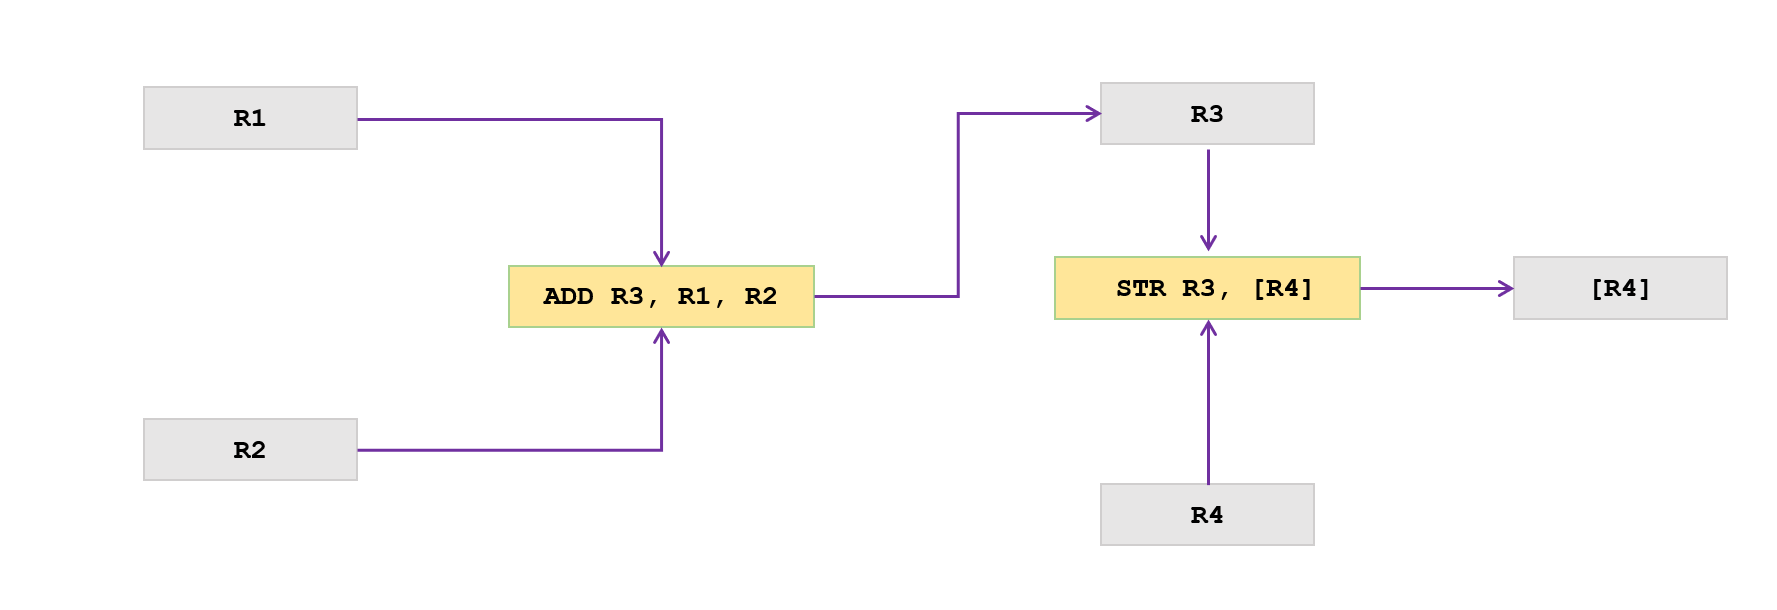
\includegraphics[width=1.0\textwidth]{./figure/UD-visual.png}
    \caption{根据\autoref{code:udchain}构建的可视化数据流动方向}
    \label{fig:viaual_udchain2}
\end{figure}
在这个链中,每个箭头代表数据流动的方向,从定义节点到使用节点,然后可能再到另一个定义节点。
根据上述分析,我们可以绘制出一个使用-定义链的简化图,如\autoref{code:viaual_udchain}所示。

\begin{lstlisting}[
    language={asm},
    caption={根据\autoref{code:udchain}构建的可视化使用——定义链},
    label={code:viaual_udchain}
]
(R1) ---> (ADD R3, R1, R2) --> (R3)
(R2) ---> (ADD R3, R1, R2) --> (R3)
(R3) ---> (STR R3, [R4])
(R4) ---> (STR R3, [R4]) ---> [R4]
\end{lstlisting}

通过分析每条新指令的语义,我们可以识别所有相关的源和目标操作数。
同时随着执行轨迹中每条新指令的解析,相应的使用和定义节点被添加到不断增长的使用-定义链中。
通过这种方式,我们可以清晰地追踪程序中各个值的来源和去向,这对于理解程序的行为以及调试和分析程序中的错误非常有帮助。

\textbf{(2)数据恢复}\ 在构建了使用-定义链后,逆向执行过程的下一步是逆向恢复每条指令执行前的寄存器值。
为了实现这一目标,我们设计了多种处理程序来处理特定类型的指令。
例如,我们为加法操作设计了$add\_handler$函数。
以指令$add R0, R1$为例,我们可以推导出以下三种关系:(1)$R0'=R0+R1$,可以获得$R0'$的值,即指令被执行后$R0$的值;
(2)$R0=R0'−R1$,可以逆向恢复执行前R0的值。
(3)$R1=R0'−R0$,可以逆向恢复R1的值。
如果在三个操作数中只有一个未知值,我们可以使用其他两个值来恢复它,并更新相应的节点。
每当使用-定义链中的一个节点被更新时,本方法会检查整个链条,寻找其他可能的更新来传播。
这个迭代过程持续进行,直到使用-定义链收敛,此时本方法已尽可能多地恢复了之前的状态。

\begin{figure}[h]
    \centering
    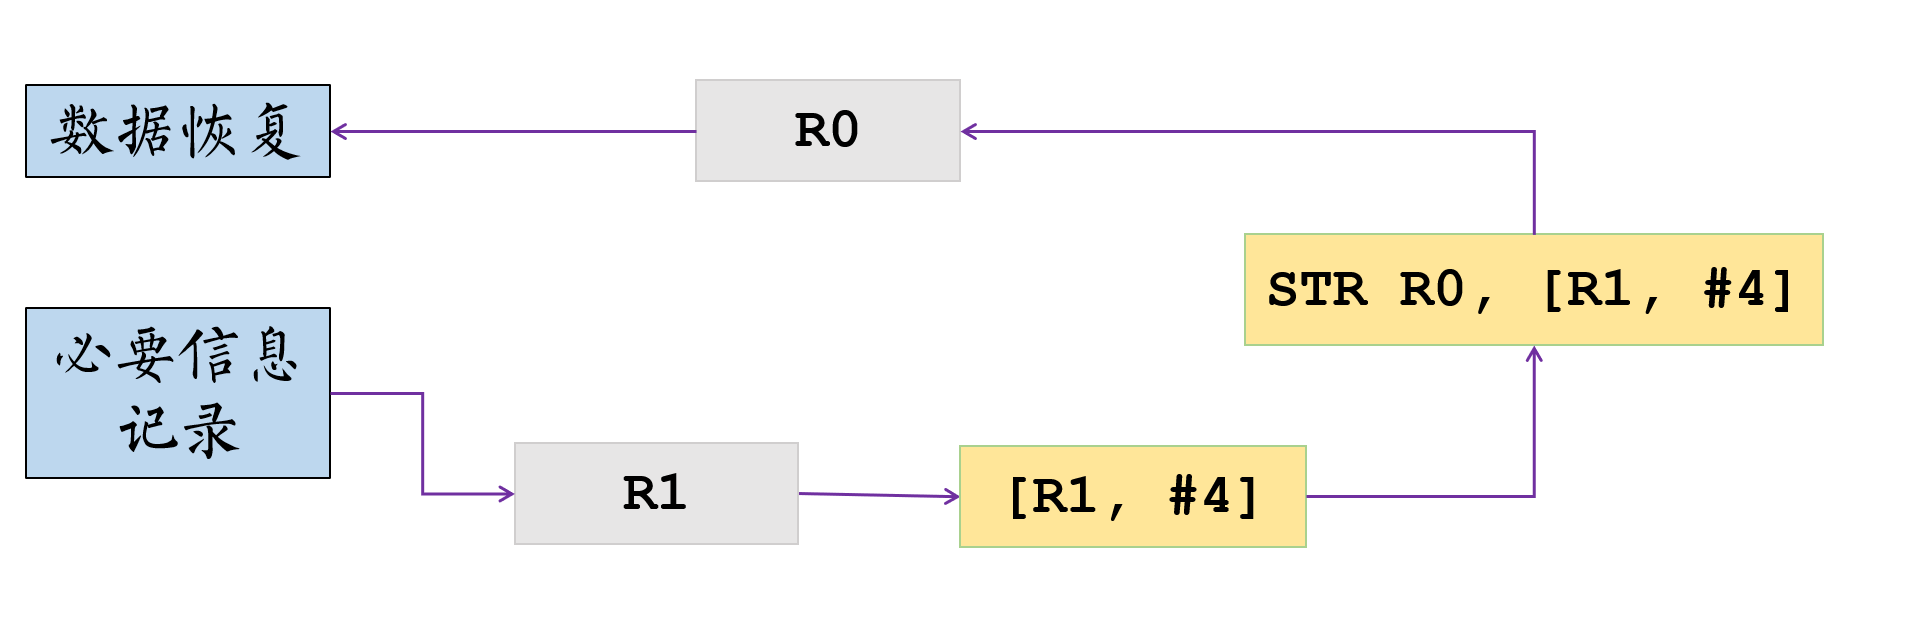
\includegraphics[width=1.0\textwidth]{./figure/solvealias.png}
    \caption{根据第一阶段记录信息恢复运行时数据示例}
    \label{fig:solvealias}
\end{figure}

值得注意的是,这种方法无法处理内存别名问题。
为了解决这个问题,我们利用第一阶段记录的信息来恢复实际的运行时数据。
例如,对于指令$STR\ R0,\ [R1,\ \#4]$,它将$R0$的值存储在地址$R1+4$的内存中。

如\autoref{fig:solvealias}所示,在之前的足迹收集阶段,我们已经获得了目标地址(即$[R1,\ \#4]$)和要存储的具体数据。
有了这个数据事件,我们可以直接从具体数据中恢复R0的值,并通过从目标地址减去4字节来恢复R1的值。
与假设测试和值集分析等其他技术相比,这种方法不仅保证了精确性,还大大加快了逆向执行的速度。
\subsubsection{根因分析}
在这一节中,我们介绍本文方法的最后一个环节——根因分析。
首先,我们从嵌入式固件崩溃处开始执行后向污点分析,以识别与根本原因相关的指令。
这一分析通过跟踪与崩溃相关的数据的污点传播,来确定可能导致崩溃的指令,
从而使分析人员可以更有效地聚焦于最关键的指令,更精确地定位和理解崩溃的原因。

本阶段主要用到的方法是后向污点分析。后向污点分析从崩溃点开始,逆向追溯数据的来源,以确定是哪些操作和值导致了程序崩溃,从而确定根因。
基于此信息,我们通过逆向执行轨迹,从崩溃点开始追踪数据的反向流动。下面将详细解释后向污点分析环节。

\textbf{(1)污点汇的定义和作用}\ 
污点汇(Taint Sink)是后向污点分析中定义的一个术语,它指的是分析的起始点,通常是内存地址或寄存器,它们直接关联到错误或异常的发生。
在内存读写错误的情况下,涉及的寄存器或内存位置成为污点汇;
如果是由特定的指令如跳转或调用导致的崩溃,涉及的寄存器(如程序计数器PC)或相关栈地址被标记为污点汇。
如果一条指令试图从一个未初始化的寄存器读取数据或写入到一个非法的内存地址,这个寄存器或内存地址就会被识别为污点汇。

\begin{lstlisting}[
    language={asm},
    caption={污点汇定义示例},
    label={code_taint}
]
xor edi, edi         
mov eax, 1234        
mov [edi], eax      
\end{lstlisting}

在后向污点分析中,我们会寻找与错误直接相关的内存地址或寄存器,这些就是所谓的污点汇。
如~\autoref{code_taint}所示,在这个简单的示例中,$edi$被清零,
而指令$mov\ [edi],\ eax$试图将$eax$寄存器中的值写入到$edi$寄存器指向的内存地址,这会导致访问违规错误。
因此在这个例子,$edi$寄存器是污点汇,
在后向污点分析过程中,我们会从$mov\ [edi],\ eax$开始,追踪导致$edi$被设为零的原因,从而揭示导致程序崩溃的根本原因。

值得注意的是,这个例子中$edi$被简单的清零来模拟非法或被保护的内存地址,
但在更为复杂的程序中,某些寄存器或内存地址可能由于错误的程序逻辑或错误的内存管理而未正确初始化或被错误地修改,从而导致了程序崩溃。

\textbf{(2)后向传播规则}\ 
本方法中,污点传播规则是用来追踪和分析程序执行过程中数据的流动,尤其是污点汇反向追踪到根因的过程。
这些规则是本方法进行后向污点分析的核心部分,帮助定位和诊断导致程序崩溃或错误行为的具体指令或操作。




\begin{lstlisting}[
    language={python},
    caption={后向污点分析算法},
    label={code_taintcode}
]
Backward_taint_analysis(crash_site, instructions):
    # 1. 利用崩溃发生的指令或位置识别污点汇
    TS = identify_taint_sinks(crash_site)
    # 2. 初始化污点集合
    taint_ins = set(TS)
    # 3. 反向追踪污点
    while taint_ins:
        # 查找当前指令的来源指令,并将其加入污点集合
        for source_ins in find(taint_ins.pop(), instructions):
            taint_ins.add(source_ins)
    # 4. 报告污点分析结果
    report_tainted_instructions(taint_ins)
\end{lstlisting}

~\autoref{code_taintcode}是后向污点分析的伪代码。
本方法中,我们从污点汇出发,使用构建好的使用-定义链追踪数据的来源。下面是污点传播的详细过程:
首先,我们根据使用定义链,识别哪些操作使用了污点汇中的数据,将污点汇转换为使用节点;
之后对于每一个使用节点,我们查找导致这些使用的定义节点,这些定义节点是之前的指令或操作,它们生成或改变了使用节点中的数据;
然后从定义节点开始,我们继续追踪这些节点的使用节点,然后再找到这些使用节点的定义节点。
这个过程是递归进行的,通过不断地追踪定义和使用的关系,
这一过程持续进行,直到没有新的节点可以添加到污点集合中,或者已追溯到数据流的起点。
这意味着所有可能与错误相关的数据流都被标识和分析了;
最后,完成污点传播后,我们集合所有的污点指令,这些指令代表了可能的错误源。通过进一步的分析,可以确定哪些指令最有可能是导致错误的根本原因。

\subsection{整体系统实现}               %3.4节
本工作伪代码如~\autoref{alg:code}所示。
\begin{table}[h]
    \centering
    \caption{物联网嵌入式固件自动化根因分析方法伪代码}
    \label{alg:code}
    \begin{tabular}{p{\linewidth}}
        \toprule
        \textbf{Algorithm}: RootCauseAnalysisOfFirmware \\
        \midrule
        \textbf{Input}: Crashing Testcase, Firmware \\
        \textbf{Output}:Root Cause Analysis Report
        \begin{algorithmic}[1]
        \Function{RCA\_F}{}
        \State $RuntimeData\ \gets\ InfoRecord(Crashing Testcase,\ Firmware)$
        \State $UD\_Chain\ \gets\ ReverseExecute$
        \State $Tainted\_ins\ \gets\ BackwardTainted(RuntimeData, UD\_Chain)$
        \State $Root\ Cause\ Analysis\ Report\ \gets\ Analysis\ and\ Report(Tainted\_ins)$
        \State \textbf{return} $Root\ Cause\ Analysis\ Report$
        \EndFunction
        \end{algorithmic} 
        \bottomrule
    \end{tabular}
\end{table}
首先,本方法接受固件二进制程序和崩溃测试用例作为输入,并以崩溃测试用例作为输入仿真执行固件二进制程序,以重现崩溃现象。
在执行过程中,通过监控内存访问和执行轨迹,收集包括具体的内存读写操作和执行的指令地址等的运行时数据;
之后进行逆向执行过程,根据收集到的数据,构建使用-定义链,用于追踪程序中的数据流和依赖关系。
同时通过逆向追踪程序执行,以识别和解析内存别名问题,精确跟踪数据依赖。
然后进行根因分析阶段,从崩溃点开始,进行后向污点分析。通过反向分析数据的流动标识和跟踪污点数据,分析可能导致崩溃的操作和指令,以确定导致崩溃的根本原因。
最后整理结果,输出详细的分析报告,包括可能的崩溃原因、关键的污点指令以及推荐的调试或修复步骤。



\subsection{本章小结}                   %3.5节
在本章中,我们概述了物联网嵌入式固件在现代技术领域中的重要性和由于安全缺陷带来的风险,并对本文主要方法设计进行了阐述。
首先我们定义了本文关注的主要问题,即无效的内存访问和无效的指令执行的问题,同时也说明了需要特别解决的内存别名问题。
之后介绍了本方法的三个主要的组件实现:高效运行时信息记录、历史信息指导的逆向执行和后向污点分析。
在高效运行时信息记录阶段,我们通过模拟执行引起崩溃的测试用例来收集关键的运行时数据。
在历史信息指导的逆向执行阶段,我们利用已收集的具体内存访问信息解决内存别名问题,确保数据流分析的准确性。
在根因分析阶段,我们通过后向污点分析确定导致崩溃的具体原因,为进一步的调查提供指导。
最后展示了我们提出的物联网嵌入式固件自动化根因分析方法的伪代码并对整个流程进行整合性说明。





%%%%%%%%%%%%%%%%%%%%%%%%%%%%%%%%%%%%%%%%%%%%%
%%%%%%%%第4章 实验与评估%%%%%%%%%%%%%%%%%%%%%%
%%%%%%%%%%%%%%%%%%%%%%%%%%%%%%%%%%%%%%%%%%%%%

\section{实验与评估}        %第4章

%%%%%%%%%%%%%%%%%%%%%%%%%%%%%%%%%%%%%%%%%%%%%
%%%%%%%%第5章 总结与展望%%%%%%%%%%%%%%%%%%%%%%
%%%%%%%%%%%%%%%%%%%%%%%%%%%%%%%%%%%%%%%%%%%%%

\section{总结与展望}        %第5章
